\documentclass[14pt, titlepage, a4paper, fleqn]{extarticle}
\usepackage{style}
\usepackage{titlepage}


\begin{document}
    \fefutitlepage{ОТЧЕТ}{к лабораторной работе по дисциплине\\ <<Дифференциальные уравнения>>} {01.03.02 <<Прикладная математика и информатика>>} {Б9121-01.03.02сп(1)}{Бабак И. А.}

    \tableofcontents

    \pagebreak

    \section{Введение}
        В этой лабораторной работе будем решать дифференциальные уравнения, определять их типы и давать характеристику (внезапно). А также решим уравнения методом Эйлера.

    \pagebreak

    \section{Задание 1: решить уравнения}
        \subsection{Постановка задачи}
            Для следующих дифференциальных уравнений указать вид, дать характеристику и найти общее решение с помощью программ компьютерной математики:

            \begin{enumerate}
                \item 
                \(y \ln{t}  = \dot{y} \cdot \ln{t^t} - \tan{\dot{y}} \cdot 
                \ln{t^{\dot{y}}}\)

                \item \(\sqrt{1 - \dot{x}^2} = \dot{x} - \sqrt{t}\)
                
                \item \(\displaystyle \dot{u}^2 - \frac{1 + \sin{2t}}{e^{2u}} = 0\)
                
                \item \(u^{\prime 3} = 1 + u\)
                
                \item \(y = 2xy' + \ln{y'}\)
            \end{enumerate}

        \subsection{Решение}
            \begin{enumerate}
                \item \(y \ln{t}  = \dot{y} \cdot \ln{t^t} - \tan{\dot{y}} \cdot 
                \ln{t^{\dot{y}}}\)

                    \(y = \dot{y}t - \dot{y} \cdot \tan{\dot{y}}\)

                    \textit{Вид уравнения:} 
                        \(F(t, ~ y, ~ \dot{y}) = 0\).

                    \textit{Характеристика уравнения:}
                        Уравнение Клеро.

                    \textit{Общее решение:} 
                        \(y = C(t - \tan{C})\)

                    \textit{Особое решение:}

                        \(
                        \left\lbrace
                        \begin{aligned}
                                &t = \tan{p} + p \cdot \sec^2{p}\\
                                &y = p(t - \tan{p})
                        \end{aligned}
                        \right . 
                        \)

                \item \(\sqrt{1 - \dot{x}^2} = \dot{x} - \sqrt{t}\)
                
                    \textit{Вид уравнения:} 
                        \(F(t, ~ \dot{x}) = 0\)

                    \textit{Характеристика уравнения:} 
                        Неразрешённое относительно производной, не содержащее функции.

                    \textit{Общее решение:}
                    \(\displaystyle \left(3x + C - t^{\frac{3}{2}}\right)^2 = (2 - t)^3\)

                \item \(\displaystyle \dot{u}^2 - \frac{1 + \sin{2t}}{e^{2u}} = 0\)
                
                        \textit{Вид уравнения:} 
                            \(F(t, ~ u, ~ \dot{u}) = 0\)

                        \textit{Характеристика уравнения:}
                            Полное неразрешённое относительно производной, приводящееся к уравнению с разделяющимися переменными
                            
                        \textit{Общее решение:}
                            \(
                                (e^u + C)^2 = 1 - \sin{2t} 
                            \)

                \item \(u^{\prime 3} = 1 + u\)
                
                        \textit{Вид уравнения:} 
                            \(F(u, ~ u') = 0\)

                        \textit{Характеристика уравнения:}
                            Неразрешённое относительно производной, не содержащее аргумента.

                        \textit{Общее решение:}
                        \(27(u + 1)^2 = 8(t + C)^3\)

                \item \(y = 2xy' + \ln{y'}\)
                
                        \textit{Вид уравнения:}
                            \(F(x, y, y') = 0\)

                        \textit{Характеристика уравнения:}
                            Уравнение Лагранжа.

                        \textit{Общее решение:}
                            \(
                                \left\lbrace
                                    \begin{aligned}
                                            &x = \frac{C}{p^2} - \frac{1}{p}\\
                                            &y = 2xp + \ln{p}
                                    \end{aligned}
                                \right .     
                            \)
            \end{enumerate}

    \section{Задание 2: решить методом Эйлера}
        \subsection{Постановка задачи}
            Разрешить следующие уравнения относительно производной и, используя метод Эйлера, найти значение функции в точке. Нарисовать график искомой функции. Реализацию решения проводить на языке <<Python>>:

            \begin{enumerate}
                \item \(\displaystyle
                    \sin\Big( e^{2x}y' + \ln\big(x^2 + y^2 + \sec{xy}\big) \Big)
                     = 1 + \tan{xy}; \quad y(0) = -\frac{\pi}{3}, ~ y(1) = ?
                \)  
                
                \item \(
                    xy' - y^2 \cdot e^{-y^2} = \sin{\pi x}; \quad y(1) = \ln{2}, 
                    ~ y(\pi) = ?
                \)
            \end{enumerate}

        \subsection{Решение}
            \begin{enumerate}
                \item \(\displaystyle
                        \sin\Big( e^{2x}y' + \ln\big(x^2 + y^2 + \sec{xy}\big) \Big)
                        = 1 + \tan{xy}; \quad y(0) = -\frac{\pi}{3}, ~ y(1) = ?
                    \) \label{ref_2_1}

                    \textit{Разрешённое уравнение:}

                        \(\displaystyle y' = \frac{\arcsin(1 + \tan{xy}) - 
                        \ln(x^2 + y^2 + \sec{xy})}{e^{2x}}\)

                    \textit{Значение функции:} \(y(1) \approx -1.091995\)

                    \begin{figure}[H]
                        \centering
                        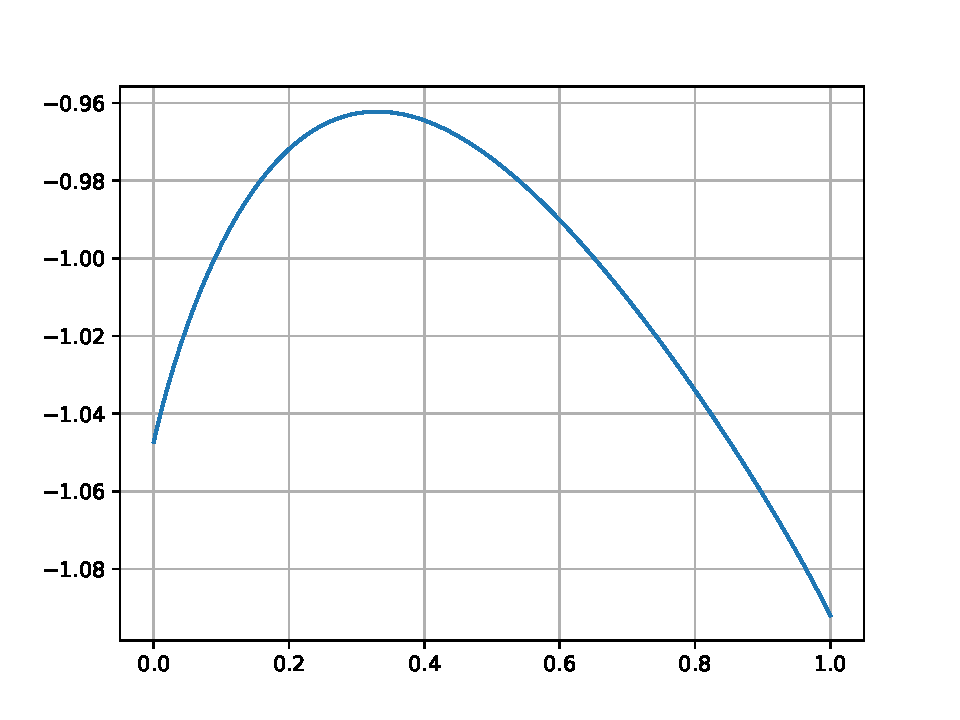
\includegraphics[width=10cm]{Figure_1.pdf}
                        \caption{График решения уравнения (\ref{ref_2_1})}
                    \end{figure}

                    \textit{Код программы:}
                        \begin{lstlisting}[
                            language=Python,                        
                            frame=lines
                        ]

import numpy as np
import matplotlib.pyplot as plt

def derivative(x, y):
    return (np.arcsin(1 + np.tan(x*y)) - np.log(x**2 + y**2 + 1 / np.cos(x*y))) / np.exp(2*x)

y_0 = -np.pi / 3
x_0 = 0
x_n = 1
h = 0.00001

xs = [x_0]
ys = [y_0]
while x_0 <= x_n:
    y_0 = derivative(x_0, y_0) * h + y_0
    x_0 += h   
    xs.append(x_0)
    ys.append(y_0)

print(f'y(1):{y_0}')
plt.plot(xs, ys)
plt.grid(True)
plt.show()
                        \end{lstlisting}

                \item \(
                    xy' - y^2 \cdot e^{-y^2} = \sin{\pi x}; \quad y(1) = \ln{2}, 
                    ~ y(\pi) = ?
                \) \label{ref_2_2}

                    \textit{Разрешённое уравнение:}
                        \(\displaystyle y' = \frac{\sin{\pi x} + y^2 \cdot e^{-y^2}}{x}\)

                    \textit{Значение функции:} \(y(\pi) \approx 0.78586\)

                    \begin{figure}[H]
                        \centering
                        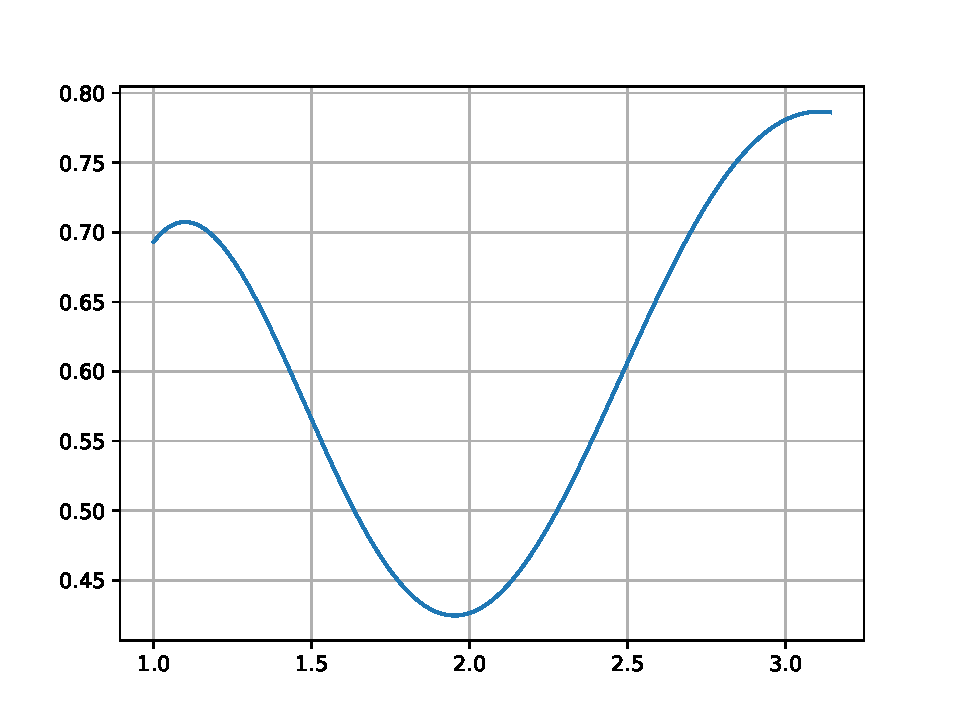
\includegraphics[width=10cm]{Figure_2.pdf}
                        \caption{График решения уравнения (\ref{ref_2_2})}
                    \end{figure}

                    \textit{Код программы:}
                        \begin{lstlisting}[
                            language=Python,                        
                            frame=lines
                        ]
import numpy as np
import matplotlib.pyplot as plt

def derivative(x, y):
    return (np.sin(np.pi * x) + y**2 * np.exp(-y**2)) / x

y_0 = np.log(2)
x_0 = 1
x_n = np.pi
h = 0.00001

xs = [x_0]
ys = [y_0]
while x_0 <= x_n:
    y_0 = derivative(x_0, y_0) * h + y_0
    x_0 += h   
    xs.append(x_0)
    ys.append(y_0)

print(f'y(pi):{y_0}')
plt.plot(xs, ys)
plt.grid(True)
plt.show()
                        \end{lstlisting}
                
            \end{enumerate}
   
    \section{Задание 3: решить уравнения}
        \subsection{Постановка задачи}
            Для следующих дифференциальных уравнений определить тип, дать характеристику и найти общее решение c помощью программ компьютерной математики:

            \begin{enumerate}
                \item \(
                    \theta^2 \ln{\theta} \cdot (r'^2 - rr'') + r^2 \ln{r} = 2\theta rr'  
                \)

                \item \(\ddot{x} + e^{2x} = 0\)
                
                \item \(tu\ddot{u} + u\dot{u} \cdot \ln{u} = t\dot{u}^2 + u\dot{u} \cdot \ln{\dot{u}}\)
            \end{enumerate}
        \subsection{Решение}
            \begin{enumerate}
                \item \(
                    \theta^2 \ln{\theta} \cdot (r'^2 - rr'') + r^2 \ln{r} = 2\theta rr'  
                \)

                    \textit{Тип уравнения:}
                        Допускающее понижение порядка.

                    \textit{Характеристика уравнения:}
                        Вполне интегрируемое уравнение.

                    \textit{Общее решение:}
                        \(\displaystyle
                            \ln{r}\ln{\theta} = C_2\theta + C_1
                        \)

                \item \(\ddot{x} + e^{2x} = 0\)
                
                    \textit{Тип уравнения:}
                        Допускающее понижение порядка.

                    \textit{Характеристика уравнения:}
                        Не содержащее независимую переменную.

                    \textit{Общее решение:}
                        \(e^{2x} = C_1^2\sech^2{\left(C_2 + tC_1\right)}\)

                \item \(tu\ddot{u} + u\dot{u} \cdot \ln{u} = t\dot{u}^2 + u\dot{u} \cdot \ln{\dot{u}}\)
                
                \textit{Тип уравнения:}
                    Допускающее понижение порядка.

                \textit{Характеристика уравнения:}
                    приводящееся к интегрируемому заменой \(\displaystyle z(t) = \frac{\dot{u}}{u}\)
                
                \textit{Общее решение:}
                    \(u = C_2e^{C_1e^t}\)
            \end{enumerate}
            
            \pagebreak

    \section{Заключение}
        В ходе лабораторной работы были выполнены поставленные задачи: уравнения решены, типы определены, характеристики даны. Рамен.

\end{document}